\\
\rule{\textwidth}{0.4pt}

\begin{verbatim}
sig timeslot{
  start   : one Int,
  end		: one Int 
}{
    //no timeslots with negative starting or ending time, and
    // a timeslot must have end after his start.
	start<=end and start > 0 and end > 0
}

//This signature represents a possible calendar task
sig task{
  time_slot : one timeslot,

//FixedTask Preferences
    car : one Bool,
    bike : one Bool,
    atm : one Bool
}{
    //At least one preference from the task' preferences is true
    (car = true or bike = true or atm = true)
}



// This signature represents a possible travel between tasks
sig travel {

//it is mandatory to specify what are the two tasks being linked by the travel
  task_from : one task,
  task_to : one task,
  time_slot : one timeslot,

//Travel mean 
//this must br unique, so only one of these can be true.
    car : one Bool,
    bike : one Bool,
    atm : one Bool

}{
    //Start and End time constraints on task_from and task_to
    task_from.time_slot.end  < task_to.time_slot.start   

    and time_slot.start >= task_from.time_slot.end         

    and time_slot.end <= task_to.time_slot.start

    //One and only one travel mean selected for a travel
    and XOR3[car, bike, atm]

}
\end{verbatim}
\hrulefill 
\\
This signature represent a possible day schedule produced by Travlendar+
note that this is not a good schedule, but only a possible one, so here
are described only the most general constraints about how a schedule has to
be
\begin{verbatim}
sig schedule{
    // this is a dummy task representing the schedule's starting point
    dummy_start_task : one task,
    
    // this is a dummy task representing the schedule's ending point
    dummy_end_task : one task,
    
    // the set of tasks complained by the schedule 
    tasks : some task,
	
    // this task serves as a reminder to the user to retake his vehicle if
    // he leave it anywhere during the day's schedule
    retake_car_task : lone task,
	
    travels: some travel  }
    
    
{
    #travels = plus[#tasks, 1]

    (no t : tasks | t = dummy_start_task)  		
																	
    (no t : tasks | t = dummy_end_task)		

    (dummy_start_task = dummy_end_task implies #tasks = 0)

    ((some tr : travels |
                tr.task_from = dummy_start_task 
                and tr.task_to = dummy_end_task ) implies
    			                                    #tasks = 0 ) 																														

    (all t : tasks | t.time_slot.start != t.time_slot.end)																											

    (all t : travels | t.time_slot.start != t.time_slot.end)
																											
    // every task is not overlapped with other tasks
    (all u :tasks | no v :tasks | 
            v != u and overlapped[v.time_slot, u.time_slot]	)
            
    (all trav : travels | no task : tasks |
        overlapped[trav.time_slot, task.time_slot])	
        
    
    (all trav : travels, u : travels |
    overlapped[trav.time_slot, u.time_slot] implies u = trav)
    
    (all t : tasks | some trav : travels | 
        trav.task_from = t and not trav.task_to = t 
        or  (
            not trav.task_from = t 
            and trav.task_to = t ))
            
    (no t : tasks | 
        t.time_slot.start <dummy_start_task.time_slot.start)
        
    (no u : tasks | 
        u.time_slot.end > dummy_end_task.time_slot.start)
        
    (all tas : tasks + dummy_end_task |
        some trav : travels |
            trav.task_to = tas)
            
            
    (all tas : tasks + dummy_start_task |
        some trav : travels | 
            trav.task_from = tas)
            
    ((no t : travels | 
        (t.car = true and t.task_from = dummy_start_task) ) implies ( 
            (no t : travels |
                t.car = true 
            ) 
            and (no t : task |
                t = retake_car_task
            )
        )
    )
    
    ((one t : travels | 
        (t.car = true and t.task_from = dummy_start_task) ) implies
            (one tas : tasks | 
                retake_car_task = tas and (one trav : travels | 
                trav.task_from = tas and retaking_car[trav, this] ) 
            or (all t :travels | t.car = true)
        )
    )
\end{verbatim}
\\
\rule{\textwidth}{0.4pt}
Here's the formal model about the world where \emph{Travlendar+} operates. This signature main goal is to constructively define the best schedule within a given set of tasks ( all tasks have to be scheduled) and a given set of travels, among which the schedule has to select the better ones. Moreover, this signature contains information about weather through a set of weather slots, which represents weather conditions during a certain time slot. Eventually, this signature contains a preferences entity which is used to model user profiles, such as the "eco friendly profile". 
\begin{verbatim}
sig World {
    // the best schedule given task preferences and weather conditions 
    bestSchedule : one schedule,
    
    // tasks for this world. bestSchedule must contain every of these tasks
    tasks : some task,
    
    // possible travels connecting each task. bestSchedule chooses one travel
    // from each task.
    travs: some travel,
    
    wtrs: some weather_slot,
    
    // general preferences. there are only 2 profiles avaiable: "eco friendly"
    // and "only car"
    prefs: one preferences
} {
    // bestSchedule must contain every of these tasks
    tasks = bestSchedule.tasks
    
    (all tr1: bestSchedule.travels | 
        one tr2 : travs | 
            tr1 = tr2 )

    // Domain assumption : all tasks are don't overlap each other
    (all t1 : tasks, t2 : tasks | 
        (t2 != t1) implies 
            ( t1.time_slot != t2.time_slot and
            not overlapped[t1.time_slot, t2.time_slot])
    ) 

    // we use two predicates to check preferences and weather conditions.
    // see predicates section for further informations. here we check these
    // predicates for each travel in bestSchedule.
    (all tr1: bestSchedule.travels | 
        (weatherCompliant[tr1 , this] and prefCompliant[tr1, prefs]))

 
    // here we assume that we want to chose the solution with as much as 
    // short travels, given the task preferences. this behaviour is just for
    // demonstration purposes, as it can be modified by other preferences that
    // are hereby not modeled.
    (all tr : bestSchedule.travels |
        no tr2 : travs | 
            ( tr != tr2 ) and (( tr.task_from = tr2.task_from )
            and (tr.task_to = tr2.task_to )
            and weatherCompliant[tr2 , this]
            and prefCompliant[tr2, prefs]
            and ( minus[tr.time_slot.end, tr.time_slot.start] >  
                minus[tr2.time_slot.end, tr2.time_slot.start] ))
    )
}
\end{verbatim}
\\
\rule{\textwidth}{0.4pt}
Eventually, here we have some other support signatures; in particular, we defined 
weather slots, temperatures (which are contained only in weather slots) and eventually some signatures representing useful boolean types that we use to check the truth value of some flags contained in the signatures discussed above.

\begin{verbatim}
sig weather_slot{
    time_slot : one timeslot,
    temperature : one temp,
	rain : one Bool
}{
}
    
sig temp {
    hot : lone Bool,
    cold : lone Bool,
    good :lone Bool
}{
    (not XOR[hot, cold]) implies good = true
}

abstract sig Bool {}

one sig true extends Bool {}
one sig false extends Bool {}

\end{verbatim}
\rule{\textwidth}{0.4pt}


\section{Support predicates}

in this section we discuss about the predicates that had been used in order to model the facts presented in the previous section. We decided to use predicates whenever there was a too complicated axiom, in order to improve readability. Moreover, we decided to use Predicates to describe widely used conditions, thus improving code reuse and reducing the model's complexity.

\begin{verbatim}
//XOR predicate
pred XOR[ x1 : Bool, x2 : Bool] {
    (x1 = false and x2 = true) or (x1 = false and x2 = true) 
}

//XOR predicate on three variables, true iif 
//only one of the passed var is true 
pred XOR3[ x1 : Bool, x2 : Bool, x3 : Bool] {

    (x1 = true and x2 = false and x3 = false) 

    or (x1 = false and x2 = true and x3 = false) 
    
    or (x1 = false and x2 = false and x3 = true)      
}

Pred prefCompliant[trav: travel, p : preferences]{

    ( trav.bike = false and trav.atm = false) implies p.ecoFriendly = false

    trav.car = false implies p.oilFriendly = false

    (trav.task_to.car = false implies trav.bike = true)

    //use bike when user prefers only car
    and ( trav.task_to.atm = false  implies trav.atm = false)

    //use bike when user prefers only atm
    and ( trav.task_to.bike = false implies trav.bike = false)
}

//not use bike when is cold, hot or raining
pred weatherCompliant[trav : travel, w : World]{

    ((some w : w.wtrs |
        (w.temperature.good = false or w.rain = true) 
        and overlapped[w.time_slot, trav.time_slot] ))
    implies	(
        trav.bike = false)

    ((some w : w.wtrs | 
        w.temperature.hot = true 
        and overlapped[w.time_slot, trav.time_slot] )) implies
    (trav.atm = false)
}

pred overlapped[t,u : timeslot]{

    u.start = t.start or
	
    (u.start > t.start implies u.start < t.end) and
	
    (t.start > u.start implies t.start < u.end) or eq[t,u]
}

pred eq[t, u: timeslot]{

    (t.start = u.start and t.end = u.end) or t=u
}

// support predicate used to check if the user's car is bringed back home when
// used.
pred retaking_car[trav : travel, s : schedule] {

    trav.car = true and (
    (some tr : s.travels | 
        (tr.task_from = trav.task_to and retaking_car[tr, s] )) 
        // there's only one travel starting from each task
	or trav.task_to = s.dummy_end_task )

}
\end{verbatim}
\section{Runnable predicates and assertions}
In this section we include all predicates that can be run in order to check whether signatures and axioms are consistent. using the world visualizer included in Alloy IDE, it is possible to verify that the model fits the Application requirements, constraints and Domain assumptions. In particular, the two "show" predicates are useful to check that world and schedule signatures are realistic. Eventually, a small collection of assertions is used to check the deductibility of some formulas from the axioms presented in the above sections.
\\
\\
\begin{verbatim}
pred showSchedule[s: schedule]{

	#s.tasks > 1
}
pred addTask[wr0 : World,  task0 : task,  wr1 : World]{

    //preconditions
    task0 != wr0.bestSchedule.dummy_start_task 
    
    task0 != wr0.bestSchedule.dummy_end_task
    
    no t : wr0.tasks | overlapped[task0.time_slot,t.time_slot]

    //postconditions
    wr1.tasks = wr0.tasks + task0
    
    some tr, tr2 : wr1.travs |
        (tr.task_from = task0 and  tr2.task_to = task0)
    
    some tr, tr2 : wr1.bestSchedule.travels |
        (tr.task_from = task0 and  tr2.task_to = task0) 
}

pred removeTask[ wr0 : World,  task0 : task,  wr1 : World]{

    //preconditions
    task0 != wr0.bestSchedule.dummy_start_task 
    
    task0 != wr0.bestSchedule.dummy_end_task
    
    one t : wr0.tasks |
	   task0 = t
	   
    //postconditions
    wr1.tasks = wr0.tasks - task0  

}


pred changeTaskPrefs[wr0 : World, task0 : task, task1 : task, wr1 : World]{

    //preconditions
    task0.time_slot = task1.time_slot and task1 != task0
    
    //postconditions
    (one wrTemp : World | 
        (removeTask[wr0, task0, wrTemp] and 
        addTask[wrTemp, task1, wr1]))  

}

assert contained{
    no s : schedule | (
        bigSchedule[s] and some x : s.tasks, y : s.tasks | (
            x.time_slot.start > y.time_slot.start 
            and x.time_slot.end < y.time_slot.end
            )
        )
}

assert continuous_sched {
    all s : schedule | (
            bigSchedule[s] implies
            one t : s.travels |
            t.task_to = s.dummy_end_task and continuous_pt2[t, s]
	)
}

//NOTE: these two predicates are needed to overcome the limitate recursive power
//of Alloy prover. in particular, the maximum recuursion depth is 4,
//but there can be schedules with more than 4 travels

pred continuous_pt2[t : travel, s :schedule]{
    t.task_from = s.dummy_start_task 
    or (some t2 : s.travels | 
        t.task_from = t2.task_to and continuous_pt3[t2, s]) 
}

pred continuous_pt3[t : travel, s :schedule]{
    t.task_from = s.dummy_start_task 
    or (some t2 : s.travels | 
        t.task_from = t2.task_to and continuous_pt2[t2, s] )

}

\end{verbatim}

\section{Proof of Consistency and Assertion checking}

here we present the result given by Alloy prover after running the above cited predicates and assertion. in this section we mainly omit the graphs given by the prover as result, because of their excessive reading complexity, given a reasonable number of instances for each signature.

\subsection{Changing task preferences}
\begin{verbatim}
run changeTaskPrefs for 
    3 World, 
    3 schedule, 
    3 weather_slot, 
    3 temp, 
    exactly 15 timeslot, 
    exactly 5 task, 
    exactly 8 travel, 
    exactly 1 preferences 
\end{verbatim}
\rule{\textwidth}{0.4pt}

\begin{figure}[H]
\centering
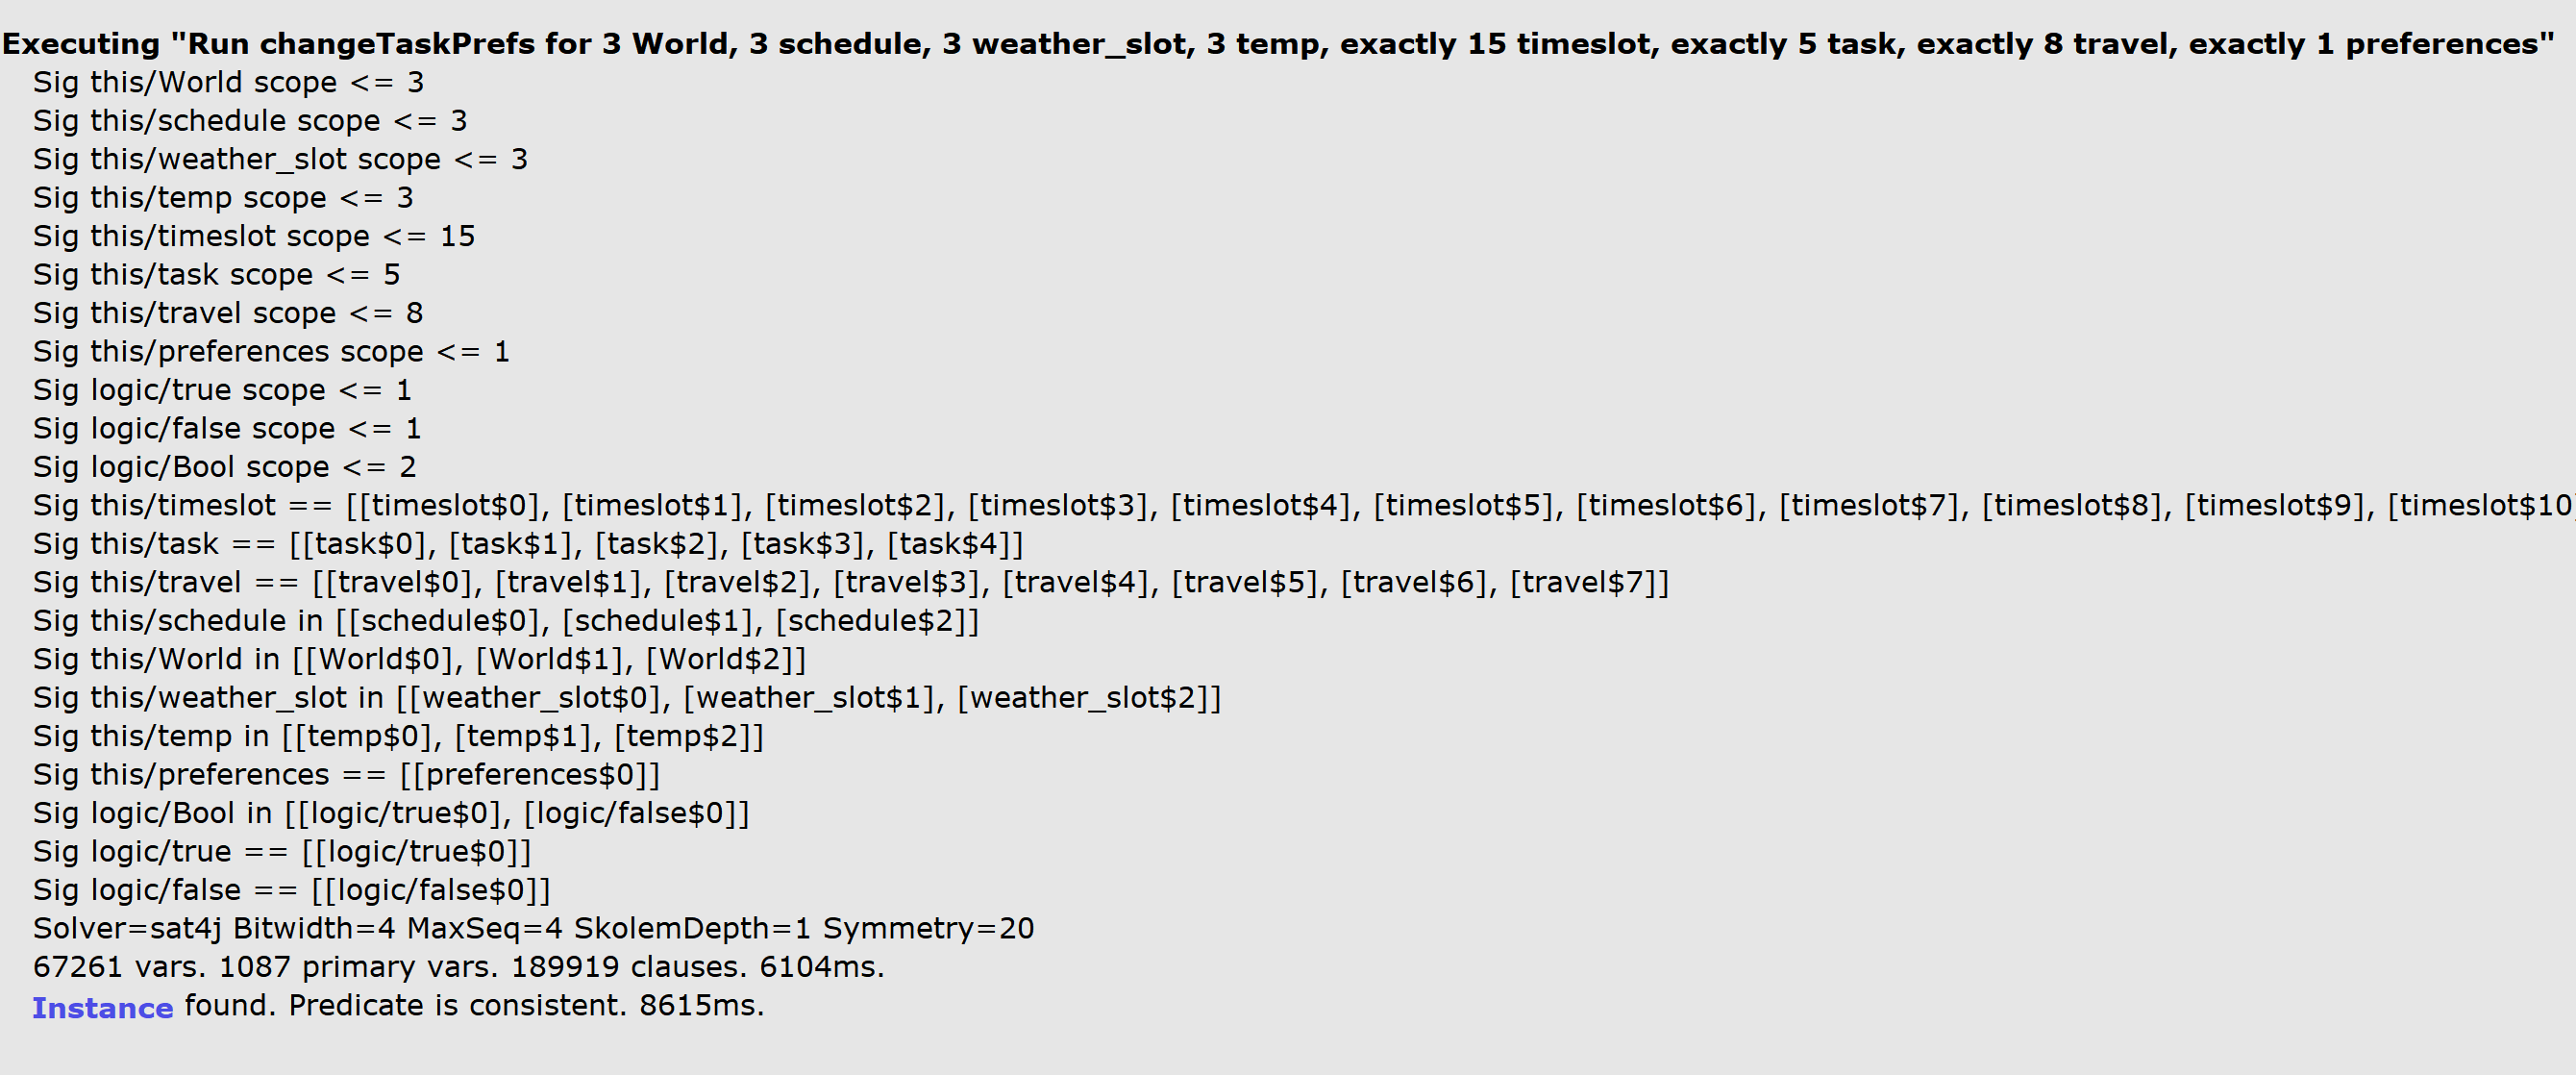
\includegraphics[scale=0.55]{Pictures/changeTaskPrefs.PNG}
\caption{Alloy Result for changeTaskPrefs. Instance is omitted, but
consistent with the non formal requirements}
\end{figure}

\subsection{Showing world}
\rule{\textwidth}{0.4pt}
\begin{verbatim}
run showWorld for 
    1 World,
    1 schedule,
    3 weather_slot,
    3 temp, 
    exactly 15 timeslot,
    exactly 4 task, 
    exactly 8 travel,
    exactly 1 preferences 
\end{verbatim}    
\rule{\textwidth}{0.4pt}

\begin{figure}[H]
\centering
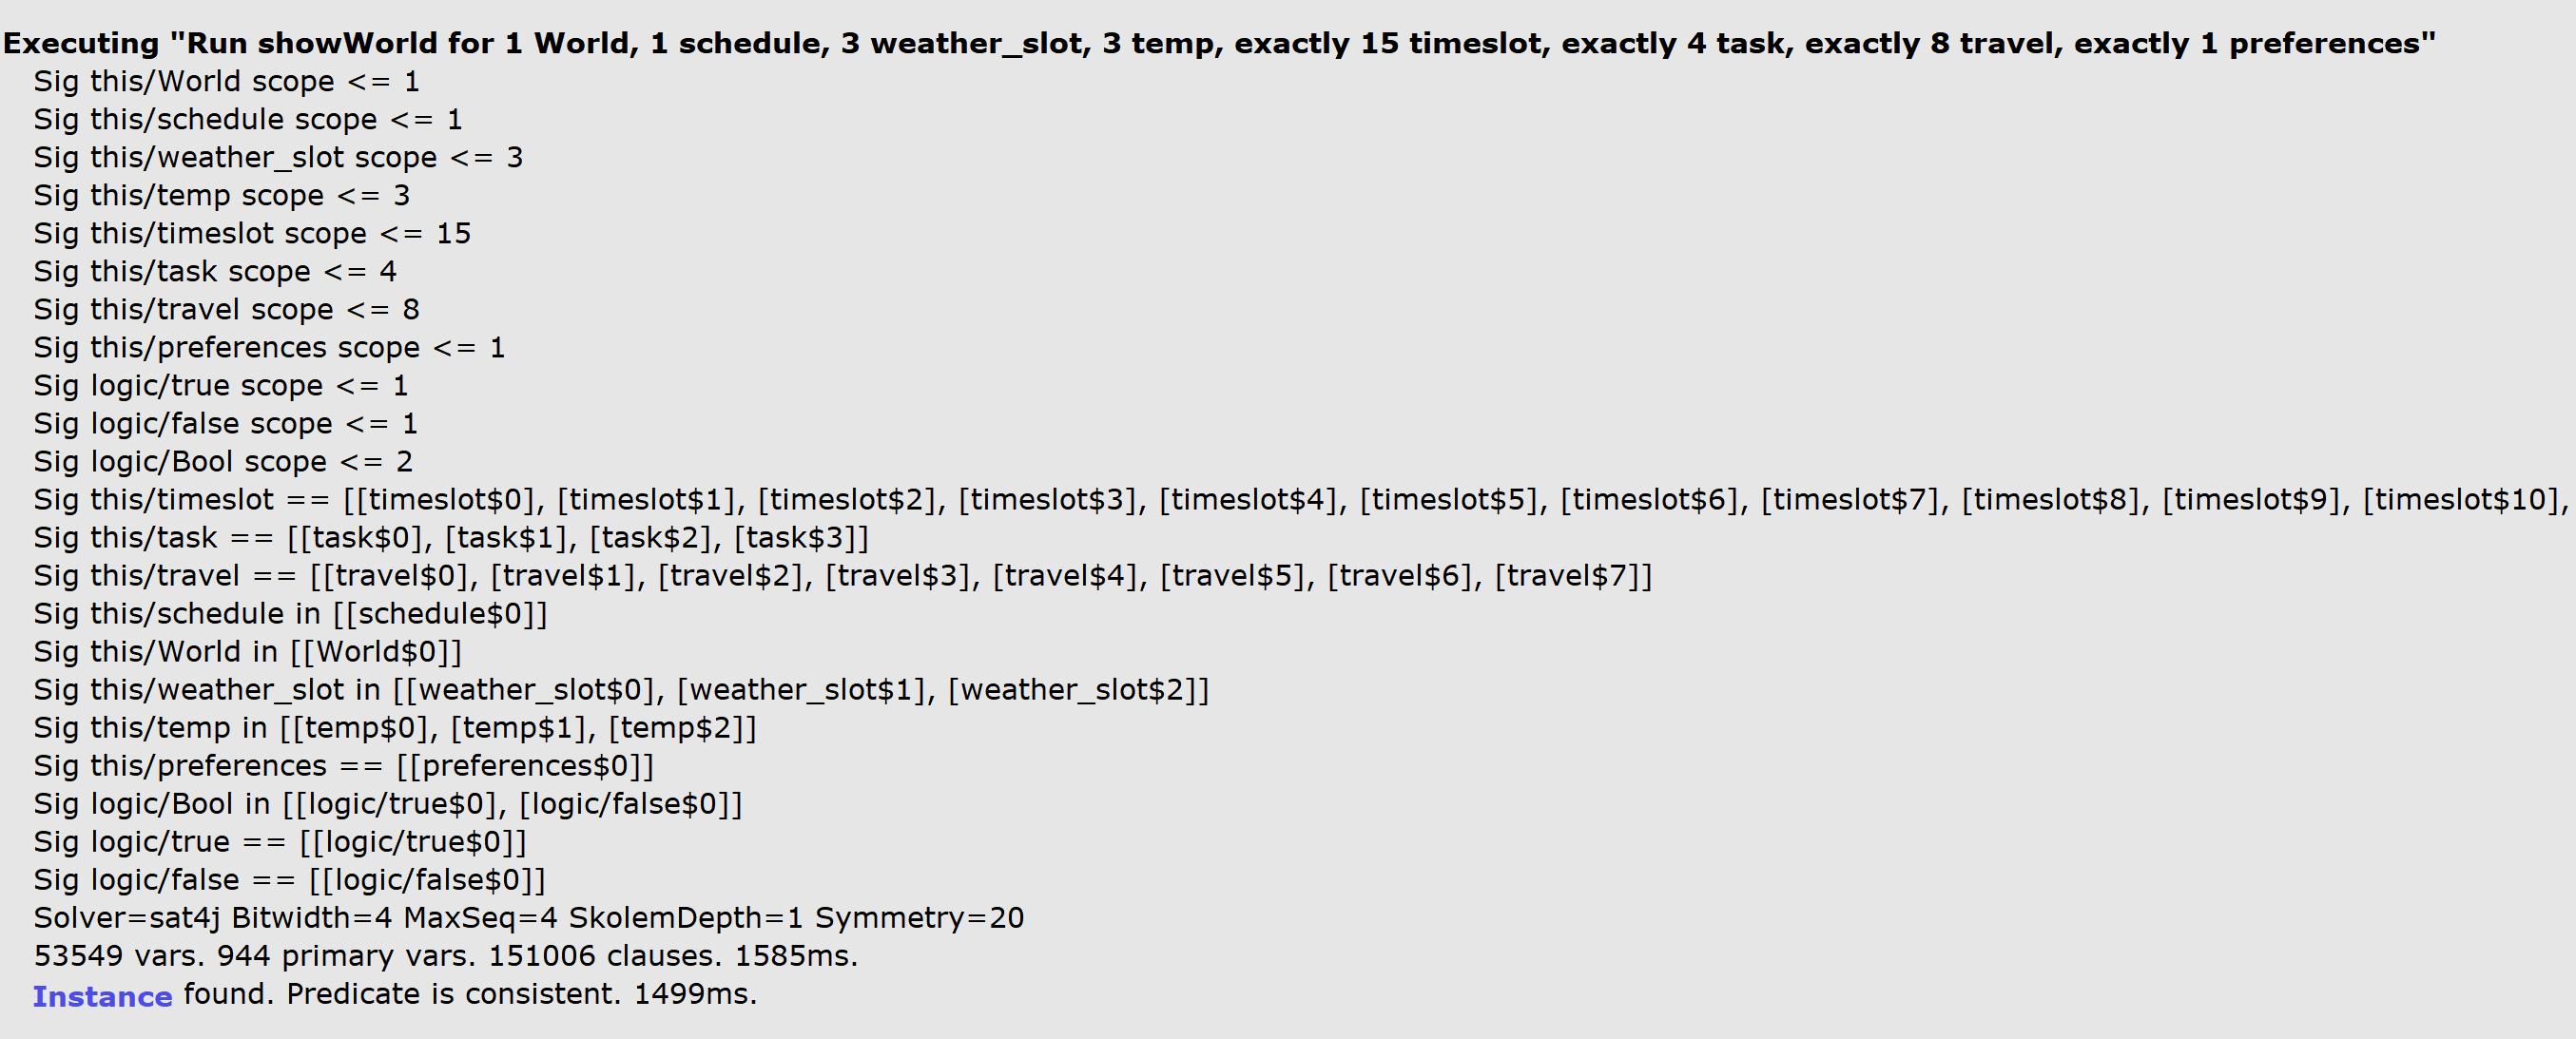
\includegraphics[scale=0.55]{Pictures/showWorld.PNG}
\caption{Alloy Result for showWorld. Instance is omitted, but
consistent with the non formal requirements}
\end{figure}

\subsection{Remove a task}
\rule{\textwidth}{0.4pt}
\begin{verbatim}
run removeTask for 
    2 World,
    2 schedule,
    3 weather_slot,
    3 temp,
    exactly 15 timeslot,
    exactly 10 task,
    exactly 12 travel,
    exactly 1 preferences     
\end{verbatim}
\rule{\textwidth}{0.4pt}

\begin{figure}[H]
\centering
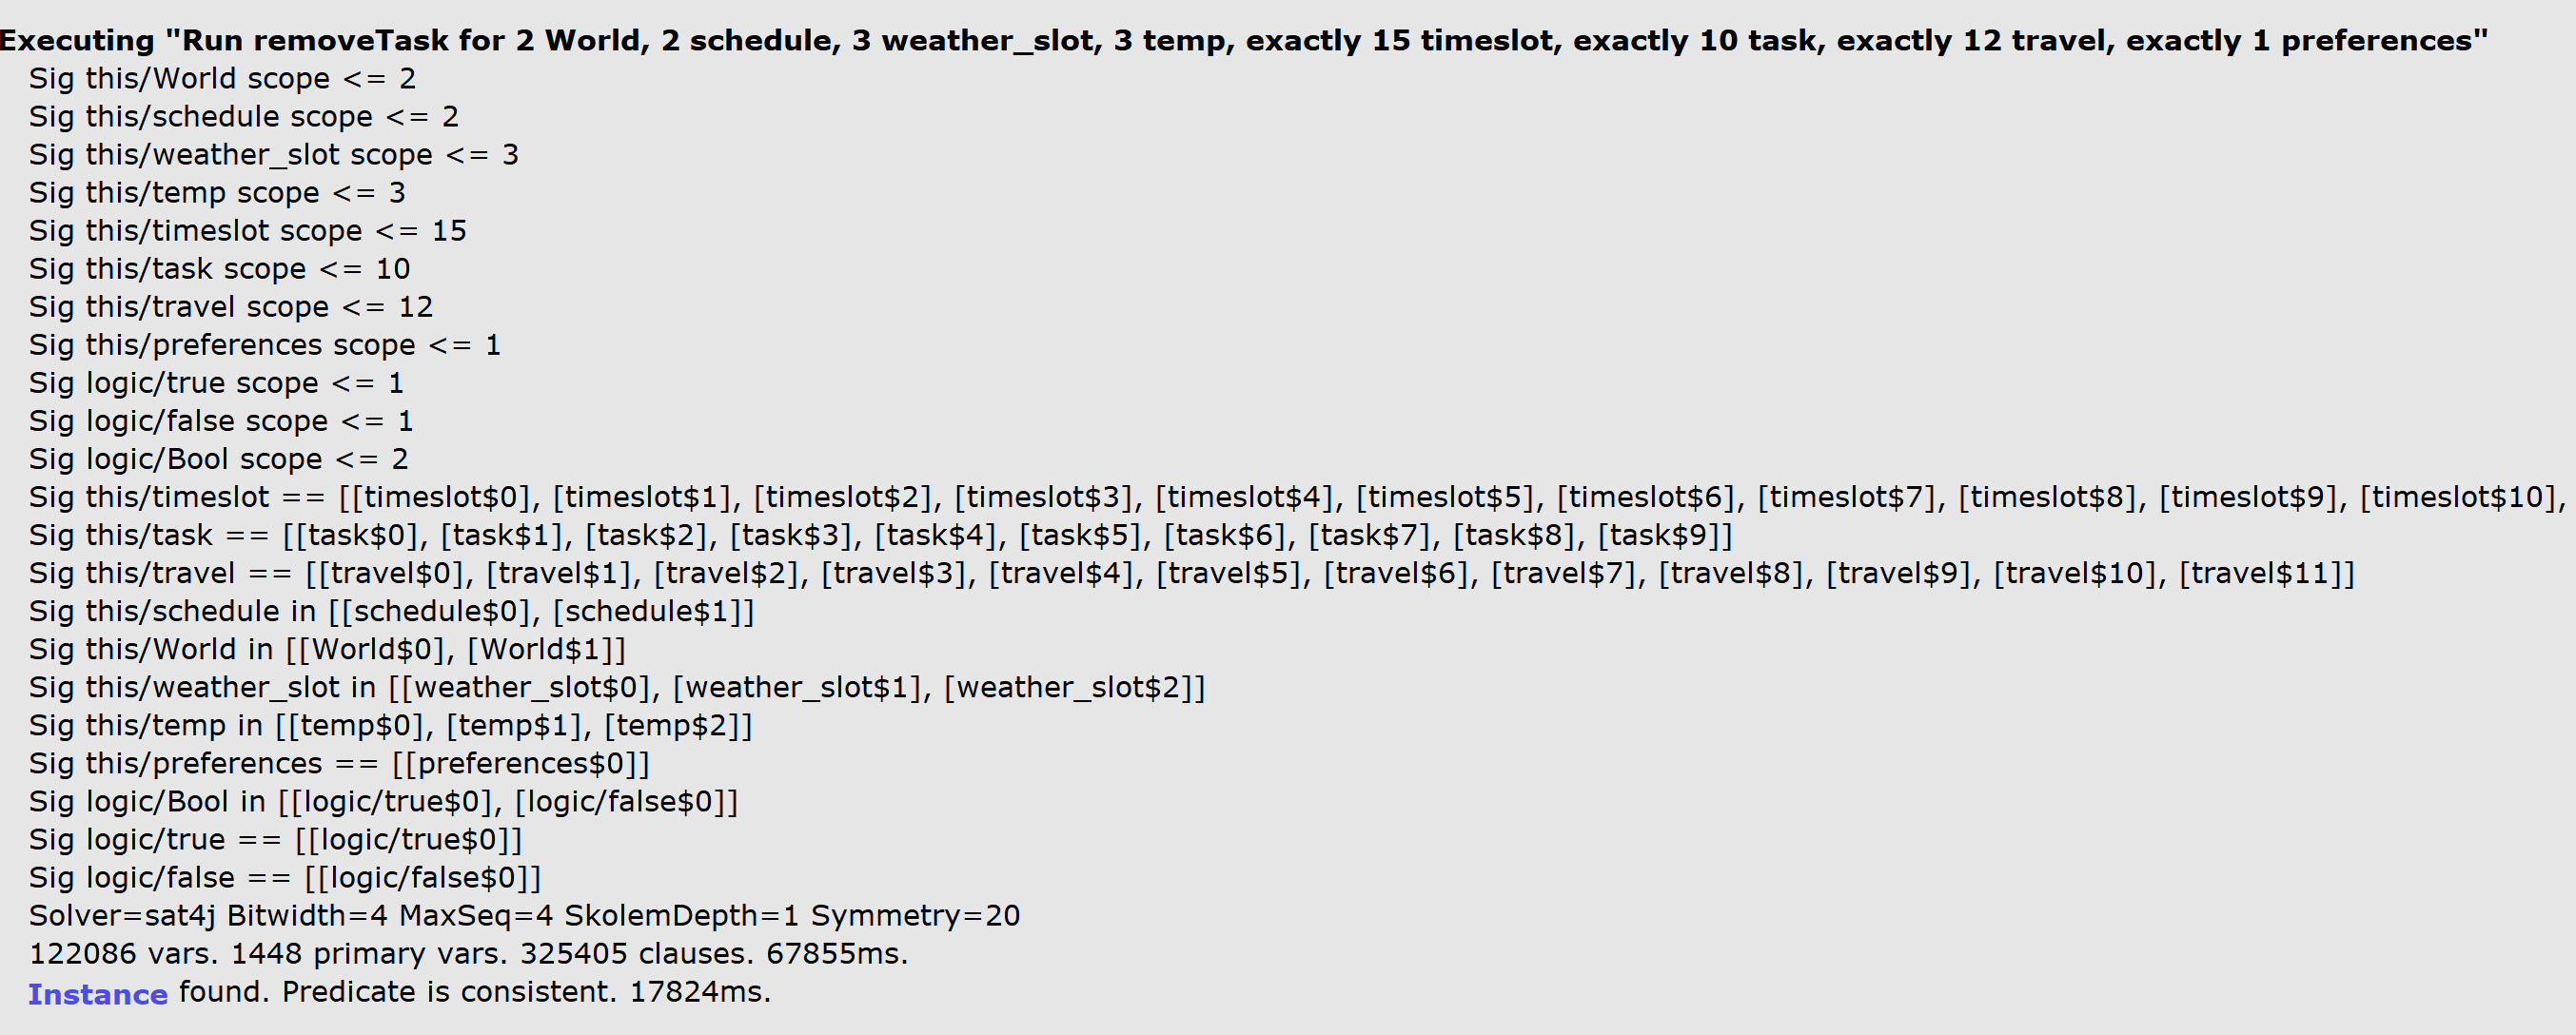
\includegraphics[scale=0.55]{Pictures/removeTask.PNG}
\caption{Alloy Result for removeTask. Instance is omitted, but
consistent with the non formal requirements}
\end{figure}
\subsection{Adding a task}
\rule{\textwidth}{0.4pt}
\begin{verbatim}
run addTask for
    2 World,
    2 schedule,
    3 weather_slot,
    3 temp,
    exactly 15 timeslot, 
    exactly 10 task,
    exactly 12 travel,
    exactly 1 preferences
\end{verbatim}
\rule{\textwidth}{0.4pt}

\begin{figure}[H]
\centering
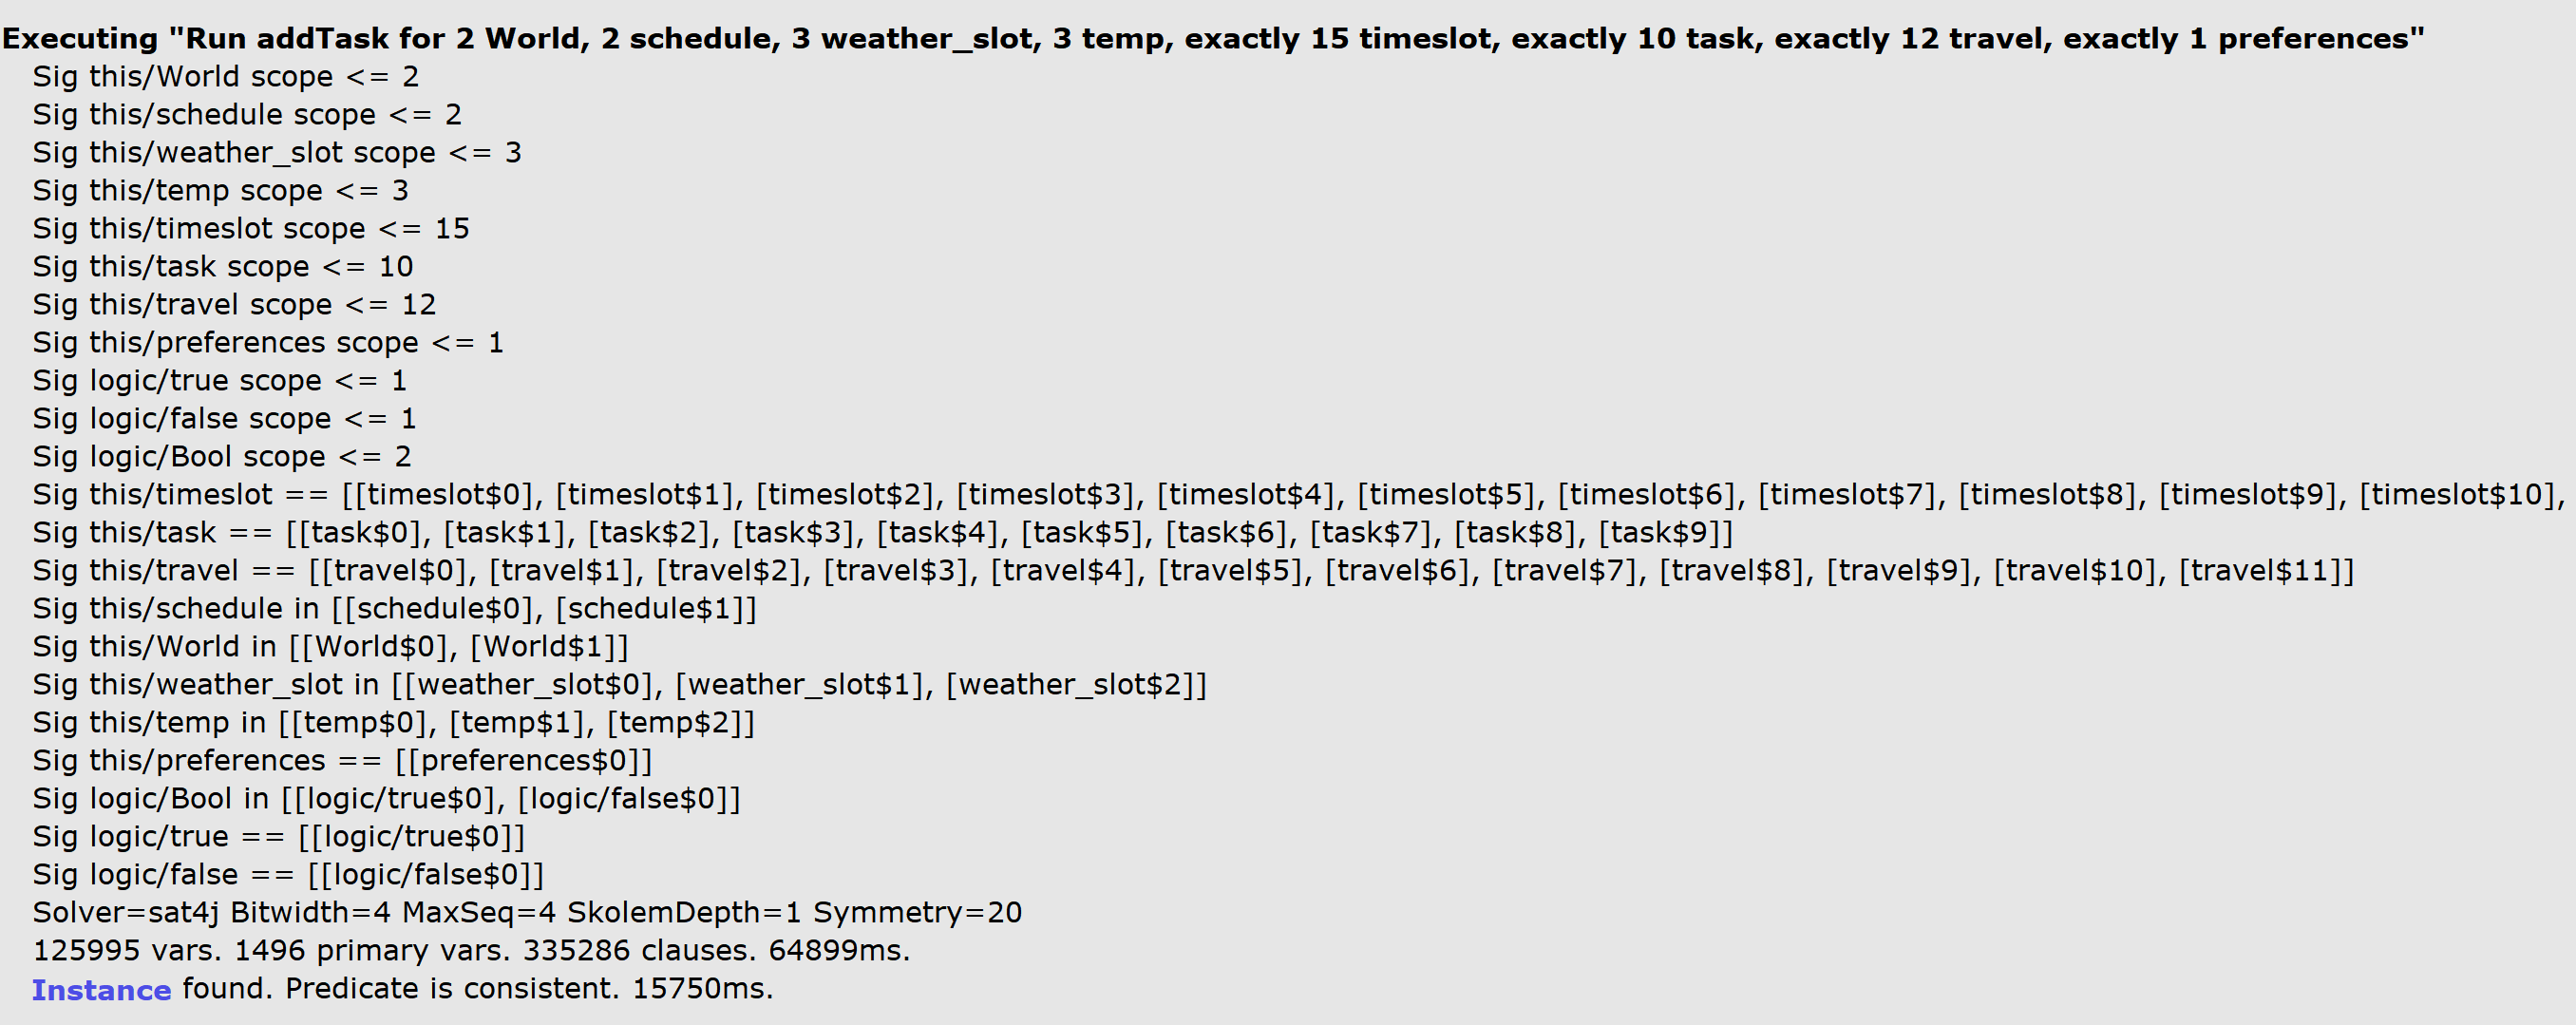
\includegraphics[scale=0.55]{Pictures/addTask.PNG}
\caption{Alloy Result for addTask. Instance is omitted, but
consistent with the non formal requirements}
\end{figure}

\rule{\textwidth}{0.4pt}
\begin{verbatim}
run showSchedule for  
    1 schedule, 
    4 task, 
    3 travel, 
    7 timeslot, 
    0 World
\end{verbatim}
\rule{\textwidth}{0.4pt}

\begin{figure}[H]
\centering
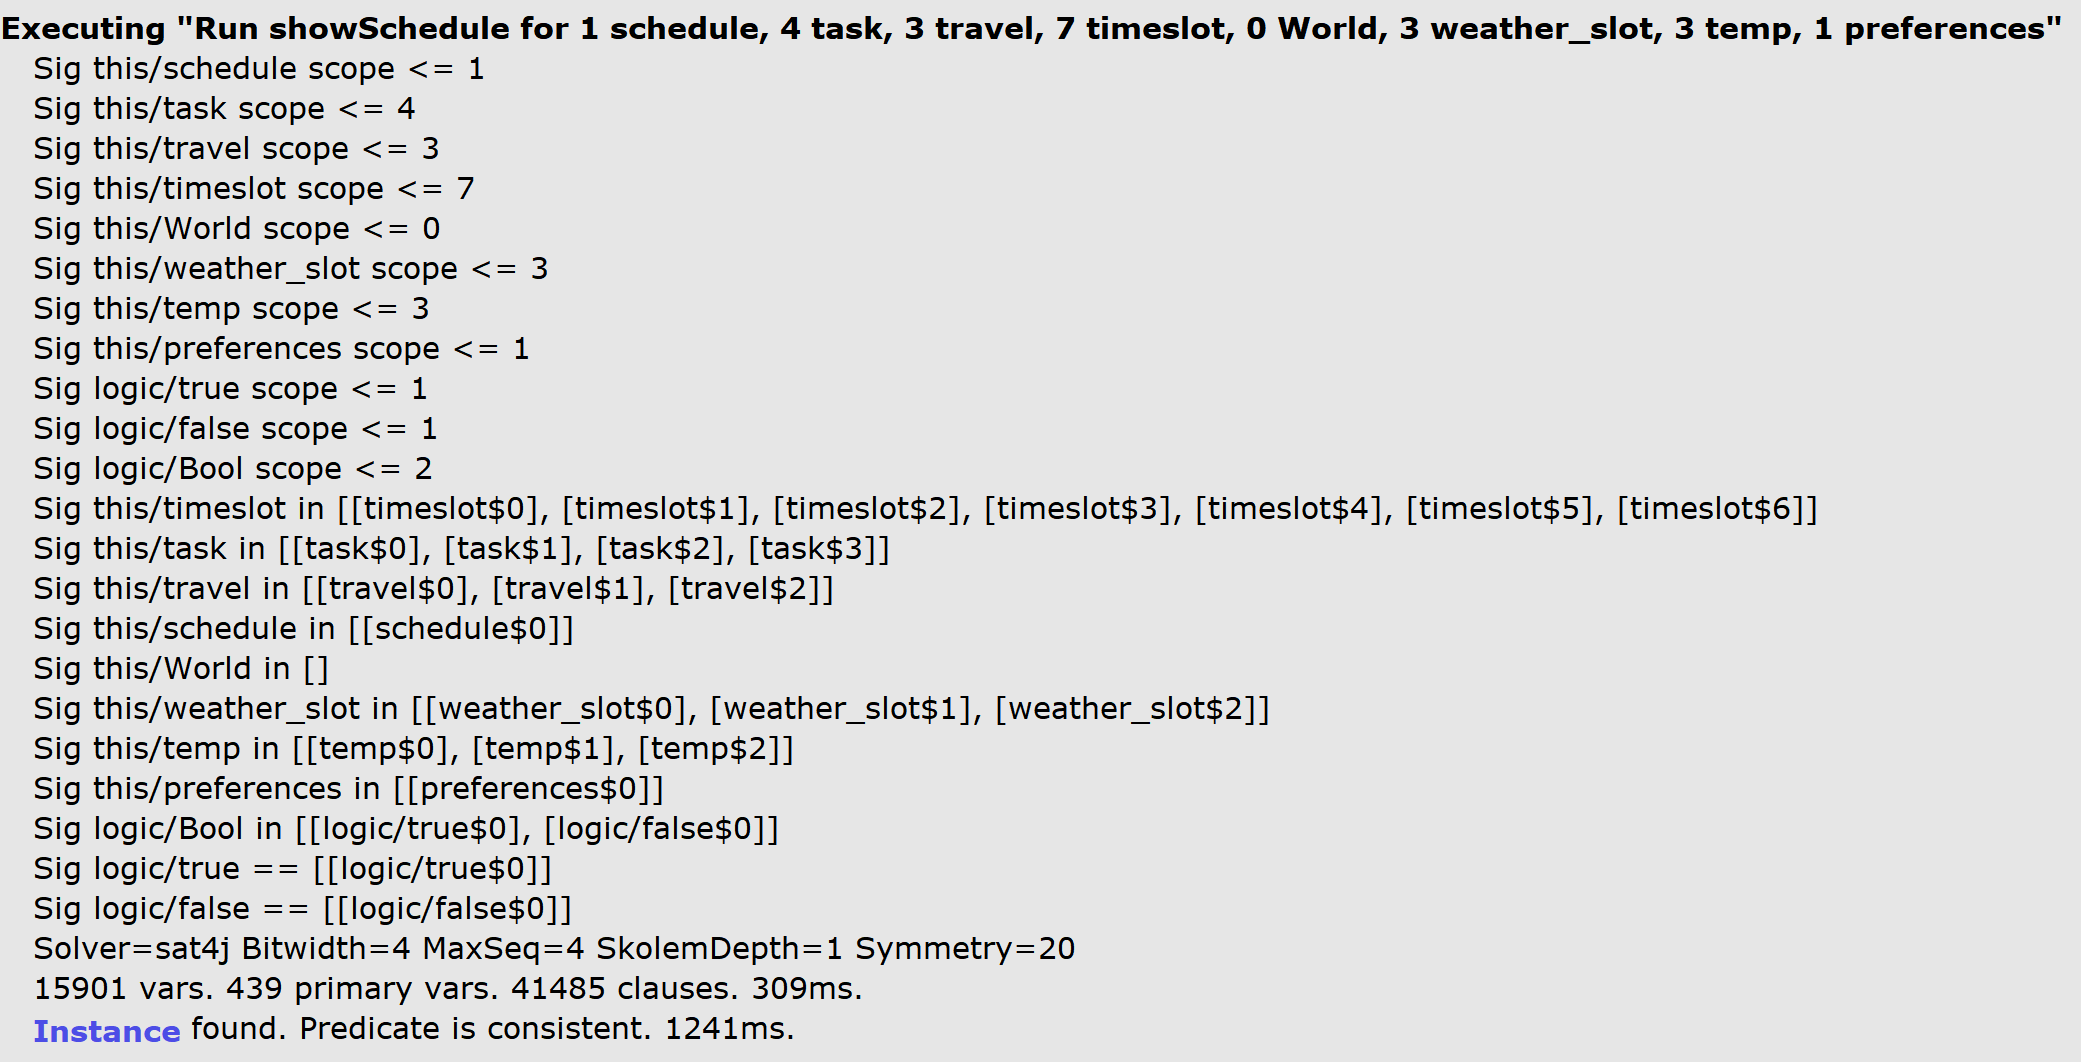
\includegraphics[scale=0.7]{Pictures/showSchedule.PNG}
\caption{Alloy Result for showSchedule. Instance is omitted, but
consistent with the non formal requirements}
\end{figure}
\subsection{Checking if a schedule is connected}
\rule{\textwidth}{0.4pt}
\begin{verbatim}
check continuous_sched for  
    1 schedule, 
    4 task, 
    3 travel, 
    7 timeslot
\end{verbatim}
\rule{\textwidth}{0.4pt}

\begin{figure}[H]
\centering
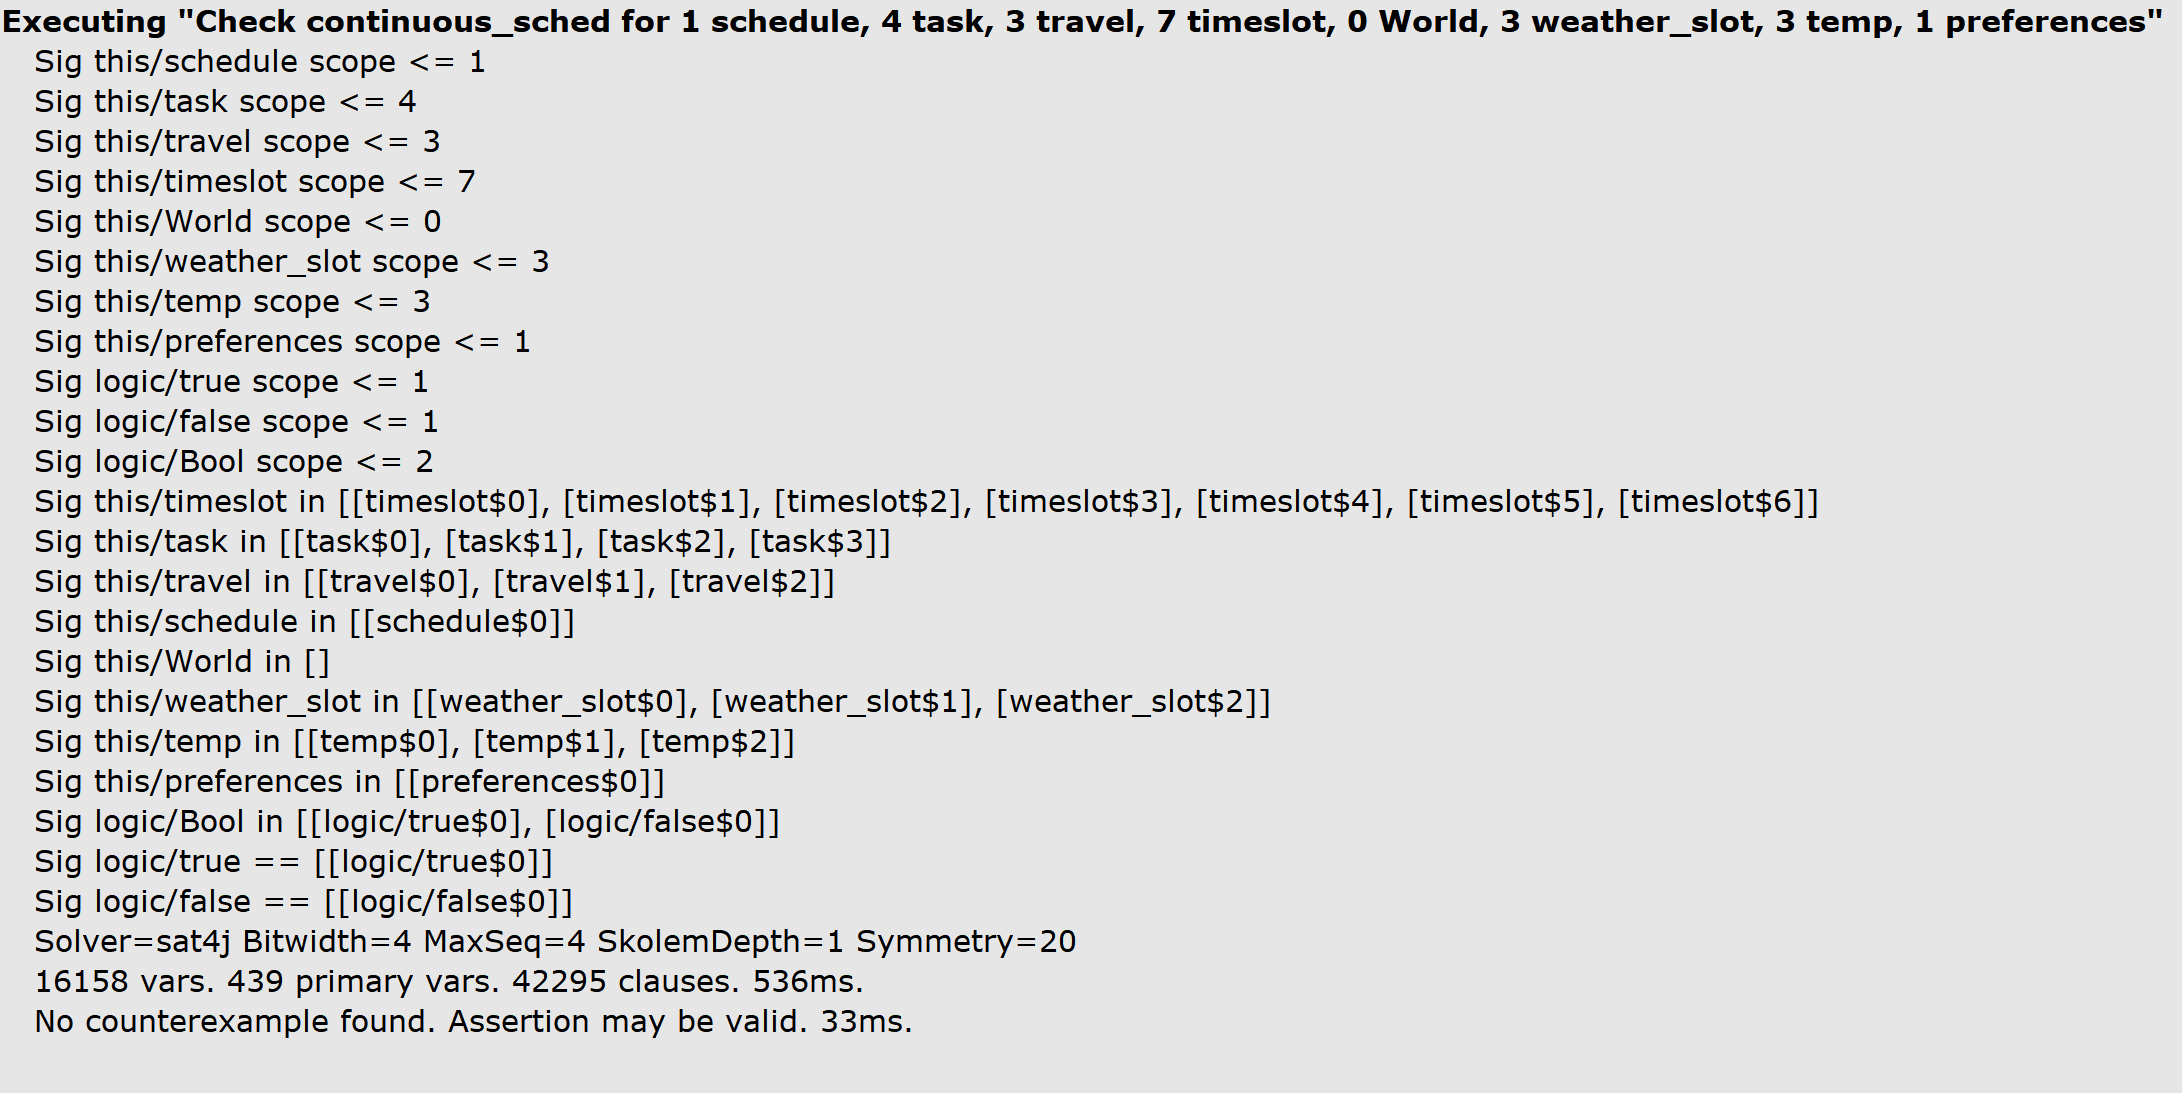
\includegraphics[scale=0.7]{Pictures/assert_continuous.PNG}
\caption{Alloy Result for continuous_sched. Instance is omitted, but
consistent with the non formal requirements}
\end{figure}
\subsection{Checking tasks not overlapped}
\rule{\textwidth}{0.4pt}
\begin{verbatim}
check contained for 
    1 schedule, 
    4 task, 
    3 travel, 
    7 timeslot
\end{verbatim}

\begin{figure}[H]
\centering
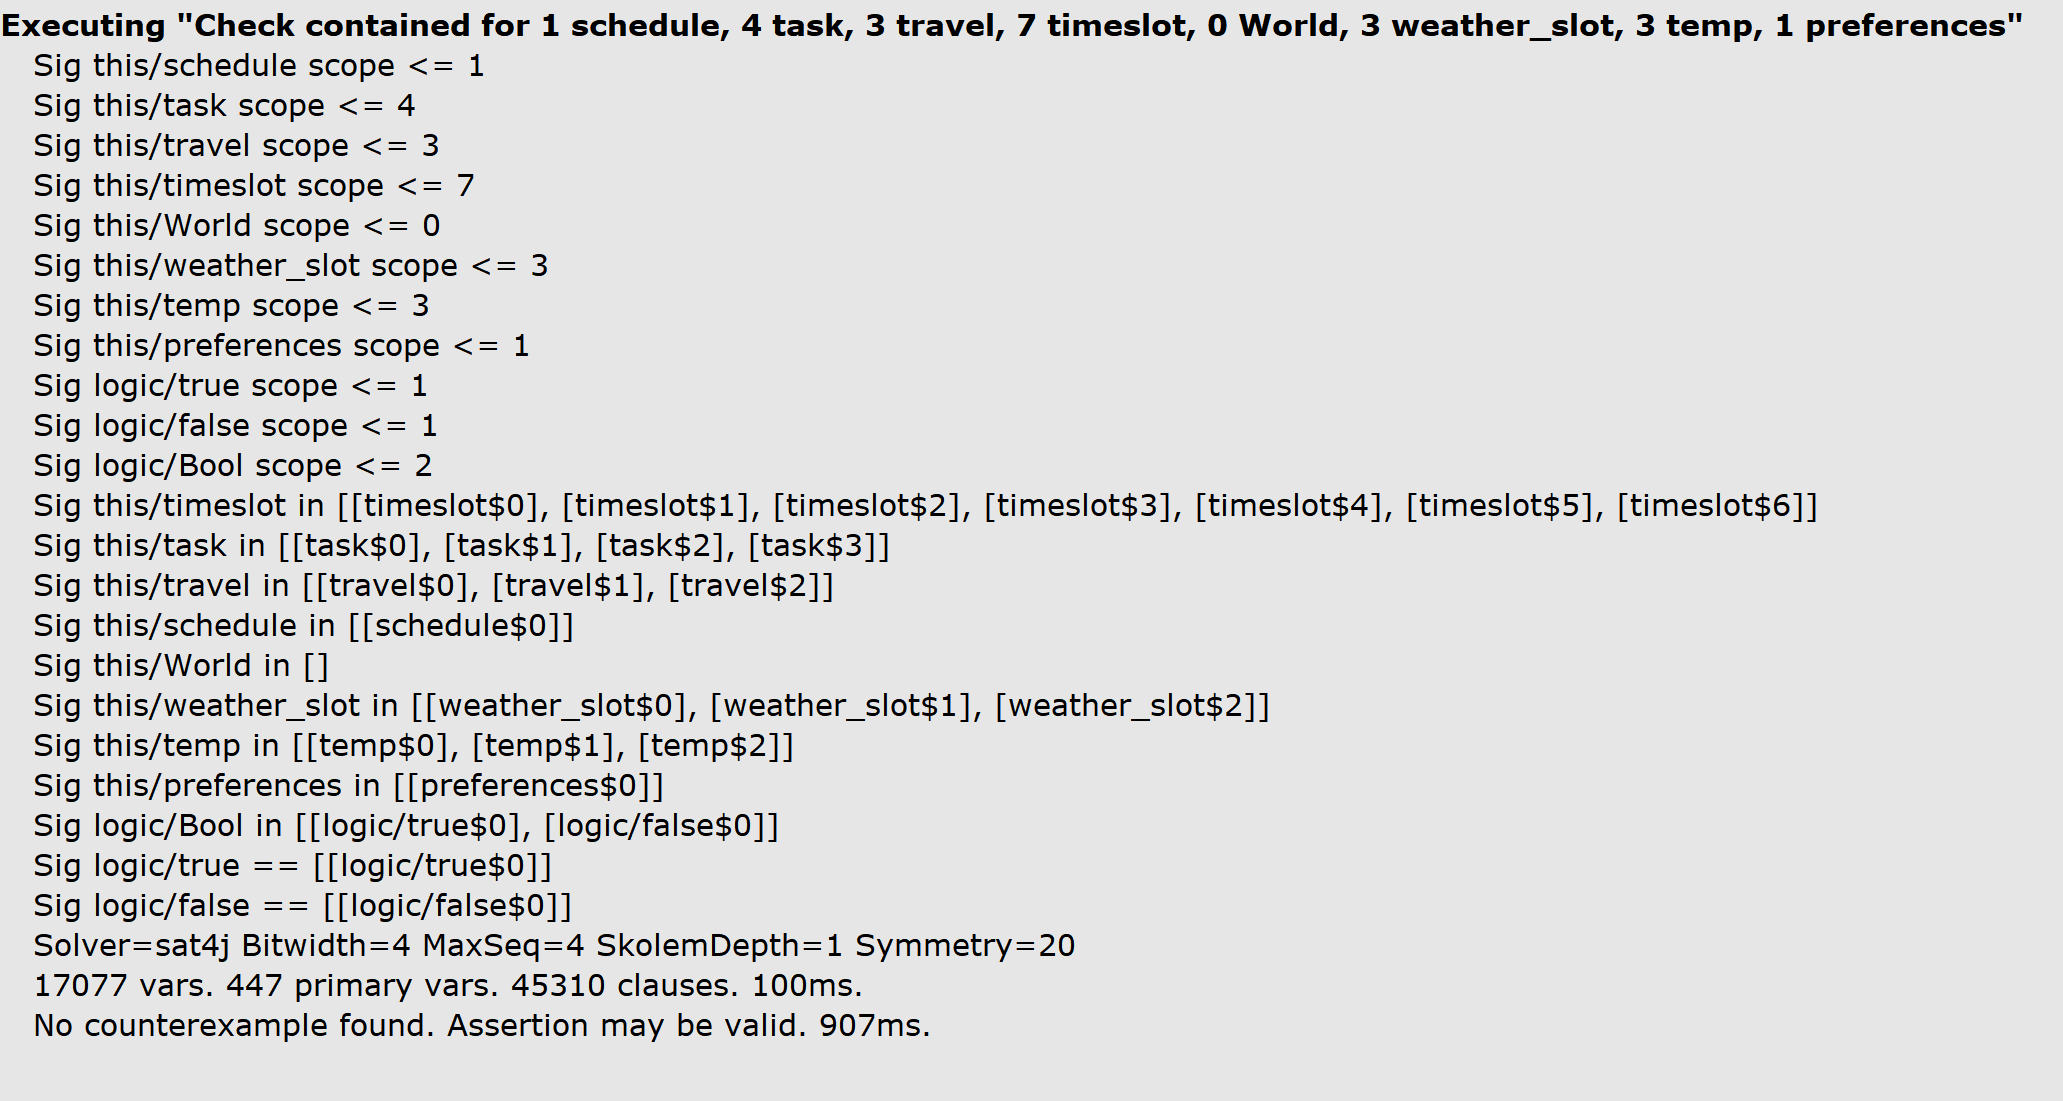
\includegraphics[scale=0.7]{Pictures/assert_noTaskContained.PNG}
\caption{Alloy Result for contained. Instance is omitted, but
consistent with the non formal requirements}
\end{figure}

